\documentclass[10pt,a4paper]{article}
\usepackage[utf8]{inputenc}
\usepackage[dutch]{babel}
\usepackage{amsmath}
\usepackage{amsfonts}
\usepackage{amssymb}
\usepackage{graphicx}
\graphicspath{ {images/} }
\usepackage{listings}
\usepackage[left=2cm,right=2cm,top=2cm,bottom=2cm]{geometry}
\author{André Jacobs | r0370664}
\title{Capita selecta: Android security}
\begin{document}
\maketitle

\section{Step 1: Application analysis}
For this first step I have chosen the application tiny flashlight
\cite{playlink1}\cite{apklink1}\\
Using apktool to decompile the apk following permissions were found in the
\texttt{AndroidManifest.xml} file:\\
\begin{figure}[h!]
  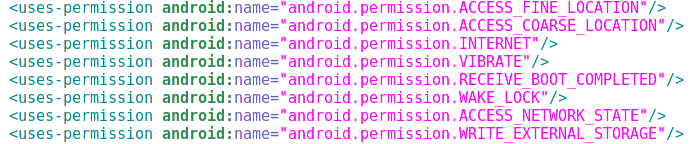
\includegraphics[width=0.7\textwidth]{manifest1}
\end{figure}

I used the included \texttt{pyparser.py} script I have written to first parse the
\texttt{ALL\_API\_CALLS.txt} file and then look through all the smali files
using a series of \texttt{grep} operations. The result of this script can be
found in the file called \texttt{result}.\\
This shows that following permissions were used:
\begin{itemize}
  \item android.permission.READ\_SMS: this seems to be used for reading
    notitications regarding download requests. This permission is not stated in
    the manifest.
  \item android.permission.CHANGE\_WIFI\_STATE: This is used to process some
    sort of transaction. This permission  is also not
    stated in the manifest.
  \item android.permission.NFC: Not stated in the manifest
  \item android.permission.VIBRATE: used by the AudioManager and
    NotificationManager of the application. This permission is requested in the
    manifest.
  \item com.android.browser.permission.READ\_HISTORY\_BOOKMARKS: not requested
  \item android.permission.CAMERA: used to access flashlight, requested in
    manifest
  \item android.permission.INTERNET: Used by http client component, requested in
    manifest
  \item android.permission.WRITE\_EXTERNAL\_STORAGE: Used by UI component and to
    save settings not requested in manifest
  \item android.permission.ACCESS\_FINE\_LOCATION: used by the LocationManager,
    probably for ads. Not requested in manifest.
  \item android.permission.KILL\_BACKGROUND\_PROCESSES: used for placing ads in
    the main UI thread. Not requested in manifest.
  \item  android.permission.READ\_PHONE\_STATE: Not requested
  \item android.permission.ACCESS\_NETWORK\_STATE: requested in manifest 
  \item android.permission.SYSTEM\_ALERT\_WINDOW: not requested in manifest 

  \item android.permission.WRITE\_SETTINGS: not requested in manifest 

  \item android.permission.WAKE\_LOCK: requested in manifest 

  
\end{itemize}

\begin{thebibliography}{9}
  
  \bibitem{playlink1}
  https://play.google.com/store/apps/details?id=com.devuni.flashlight\&utm\_source=www.apk4fun.com

  \bibitem{apklink1}
  https://www.apk4fun.com/apk/1823/
\end{thebibliography}
\end{document}
